\chapter{\textbf{Технологический раздел}}

\hfill

В соответствии с выбранной задачей -- визуализацией взрыва. Необходимо выбрать средства реализации, создать интерфейс и структуры программного обеспечения, описать ограничения и порядок работы программы. 

\section{\textbf{Выбор и обоснование языка программирования }}

Для выполнения проекта был выбран язык программирования C++/QT.

C++ -- компилируемый, статически типизированный язык программирования общего назначения \cite{c++}. 

C++ сочетает свойства высокоуровневого и низкоуровневого языка. В сравнении с его предшественником, языком C, присутствует поддержка объектно-ориентированного программирования.

Являясь одним из самых популярных языков программирования, C++ широко используется для разработки программного обеспечения \cite{usingc++}. 

Qt -- кроссплатформенная библиотека разработки GUI на С++ \cite{qt}.

Библиотека Qt является безусловным лидером среди имеющихся средств разработки кроссплатформенных приложений на языке C++. Qt – полностью объектно-ориентированная библиотека.

Все элементы в окне программы, кнопки, переключатели - это отдельные виджеты. Именно виджеты являются основой построения графических интерфейсов. С точки зрения программы, они воспринимают все
события и генерируют сигналы, которые в свою очередь вызывают слоты – специальные функции, реагирующие на различные события в окне. 

Qt прекрасно документирована, благодаря чему всегда можно найти о ней любую интересующую информацию.

Для написания программного кода использовался Qt Creator 4.8.1. Основная задача Qt Creator -- упростить разработку приложения с помощью фреймворка Qt на различных платформах.

\section{\textbf{Интерфейс пользователя }}

Взаимодействие пользователя с приложением осуществляется через интерфейс, представленный на рисунке \ref{img:interface}. 

\begin{figure}[H]
	\centering
	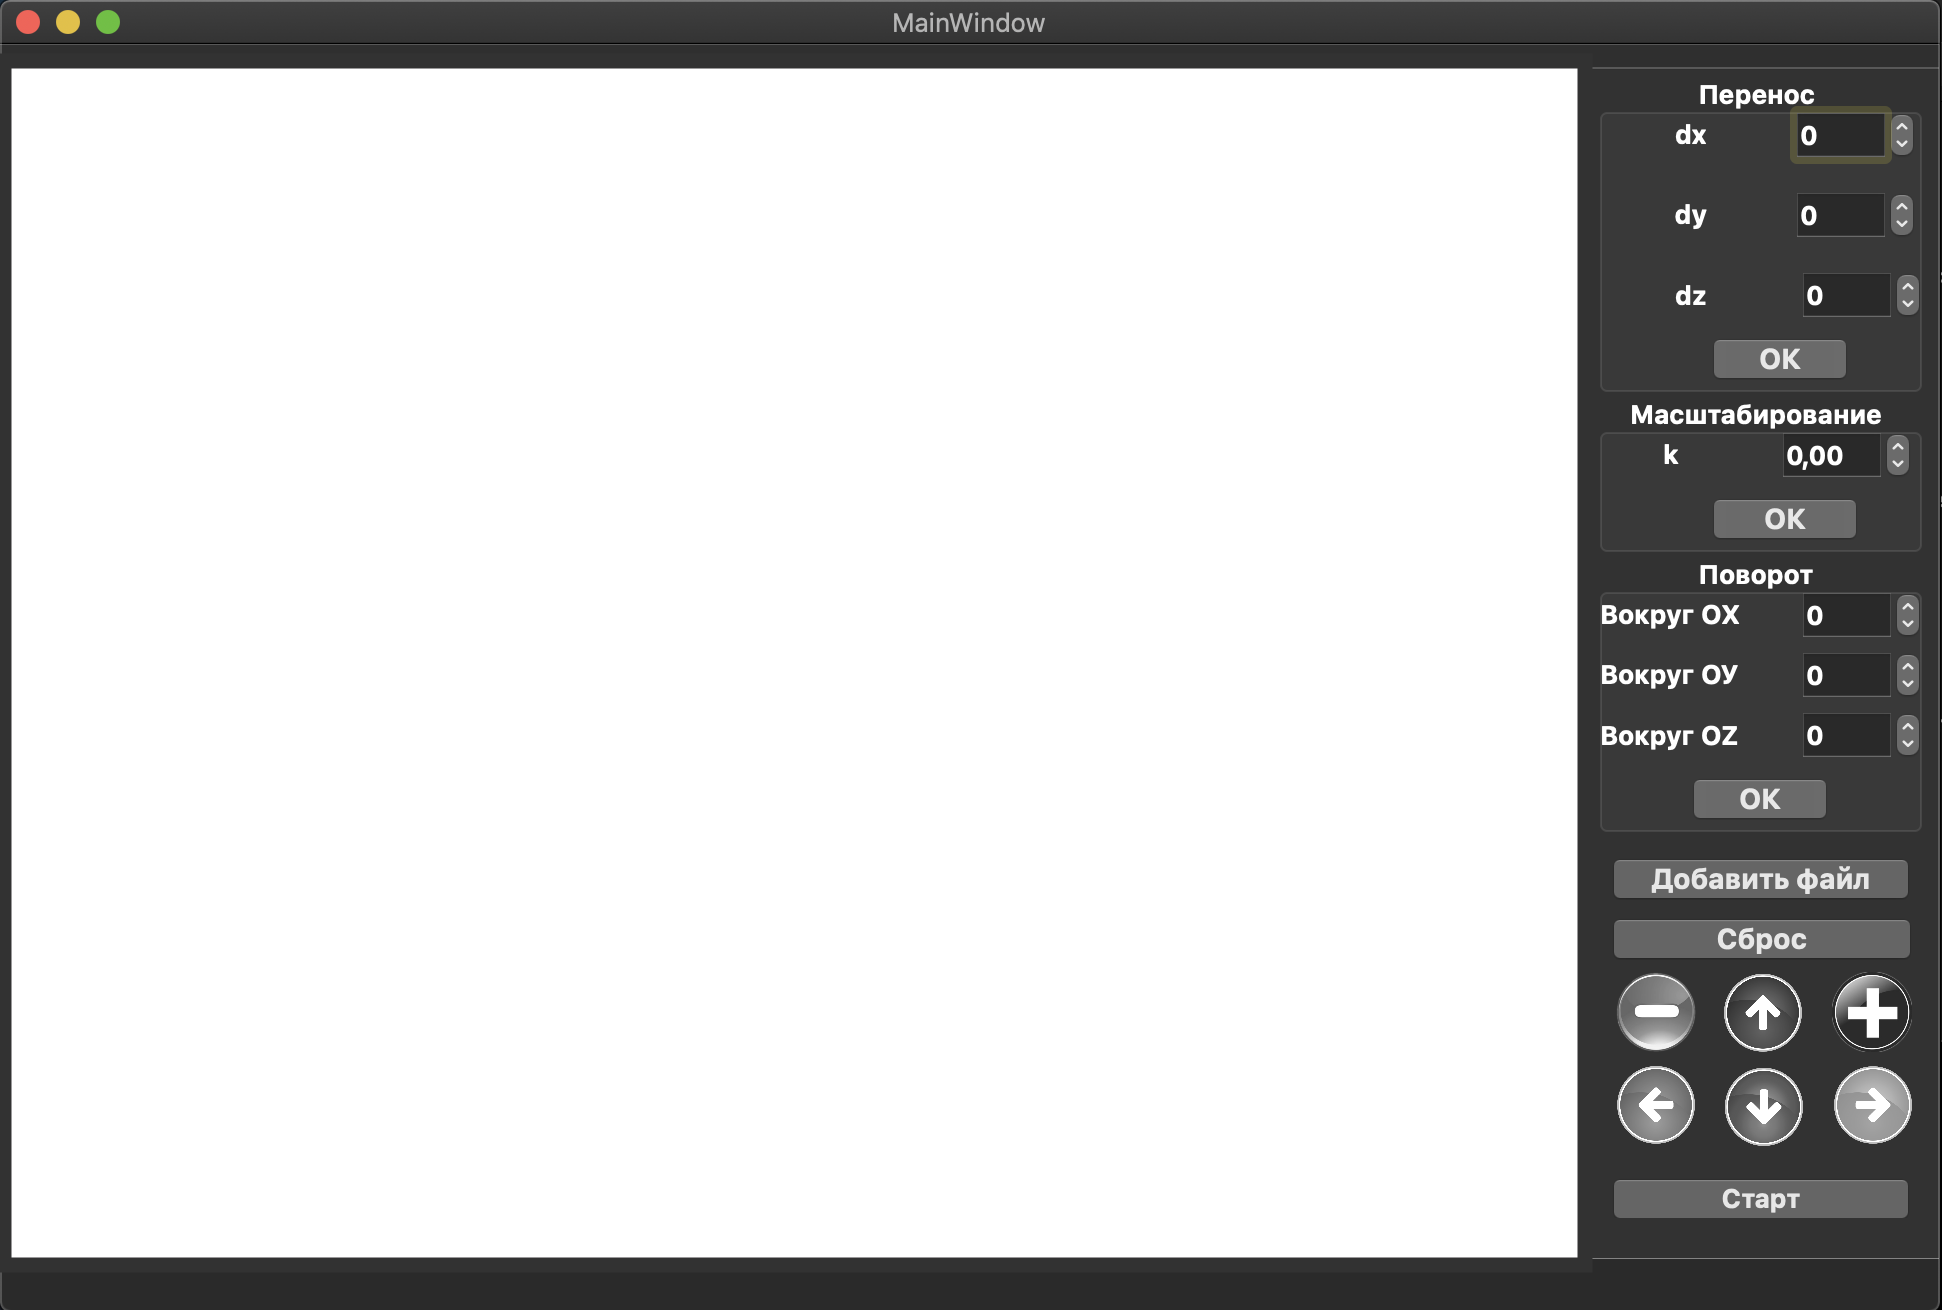
\includegraphics[scale=0.4]{interface}
	\caption{Интерфейс пользователя}
	\label{img:interface}
\end{figure}

\begin{enumerate}
	\item Доступны поля для ввода данных, при желании менять расположение и вид объектов. 
	\item Кнопки ($\to, \leftarrow, \uparrow, \downarrow, +, -$) предназначены для взаимодействия с камерой. 
	\item Кнопка  <<Сброс>> -- сбрасывает все настройки в начальное состояние. 
	\item Кнопка <<Добавить файл>> -- для загрузки данных. 
	\item Кнопка <<Старт>> -- запускает визуализацию взрыва.   
\end{enumerate}

\section{\textbf{Хранение и обмен данными в системе }}

Данные считываются из файла, содержащего в себе:

1-я строка -- количество частиц

2 -я строка и последующие строки содержать в себе информацию о частицах: положение, радиус и вес (5 значений через пробел). 

Последняя строчка рассматривается, как частица, которая в начальный момент получит скорость движения. 

Из каждого файла считывается модель, состоящая из вектора частиц, позиции земли (плоскости ограничивающей взаимодействие). Класс частицы представлен в листинге \ref{lst:particle}. 


\begin{lstlisting}[caption=Класс частицы, label = lst:particle, style=simplecode]
class Particle
{
public:
    Particle() {}
    Particle(Point_3d point, int r, int m);
    Particle(Point_3d point, int r);
    Particle(Point_3d point);
    ~Particle() {}

    void set_p(const Point_3d p);
    Point_3d get_p() const;

    void set_v(const Point_3d v);
    Point_3d get_v() const;

    void set_m(const double m);
    double get_m() const;

    void set_r(const int r);
    int get_r() const;

    void collision(Particle &p);
    void update(int time);

private:
    Point_3d point;
    Point_3d speed;
    int m;
    int radius;
};
\end{lstlisting}

\section{\textbf{Разработка программы}}

В данной работе, используется объектно-ориентированный подход программирования и паттерны проектирования\cite{patterns}. 

Для связание интерфейса и реализации используются паттерны фасад и команда. См. рисунки \ref{img:facade}, \ref{img:commands}. 

\begin{figure}[H]
	\centering
	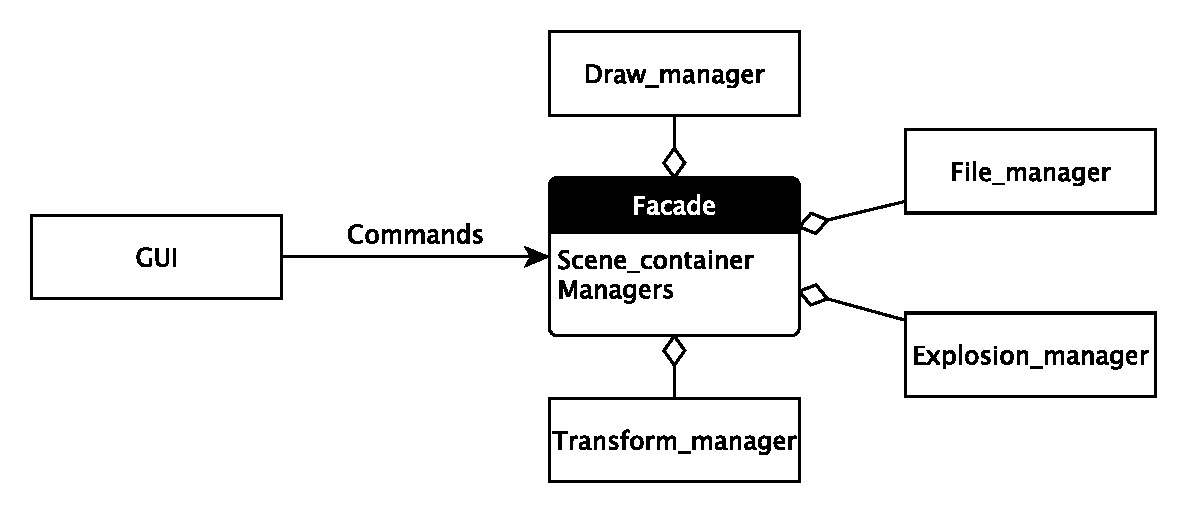
\includegraphics[scale=0.7]{facade.pdf}
	\caption{Паттерн фасад}
	\label{img:facade}
\end{figure}

\begin{figure}[H]
	\centering
	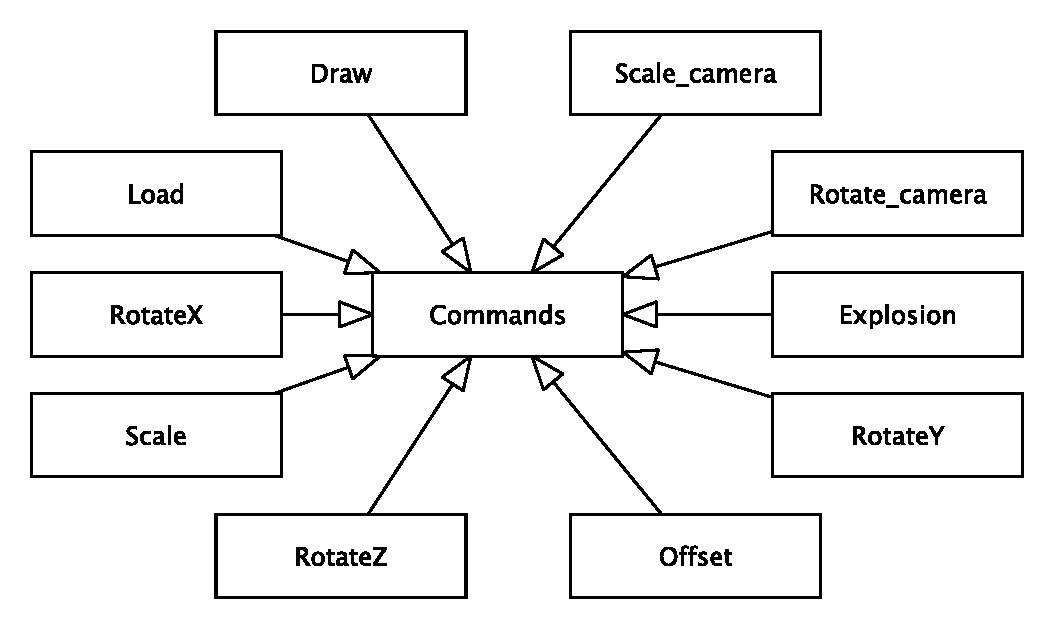
\includegraphics[scale=0.7]{commands.pdf}
	\caption{Паттер команда}
	\label{img:commands}
\end{figure}

Структура сцены в данной работе представлена на рисунке \ref{img:scenecontainer}. 

\begin{figure}[H]
	\centering
	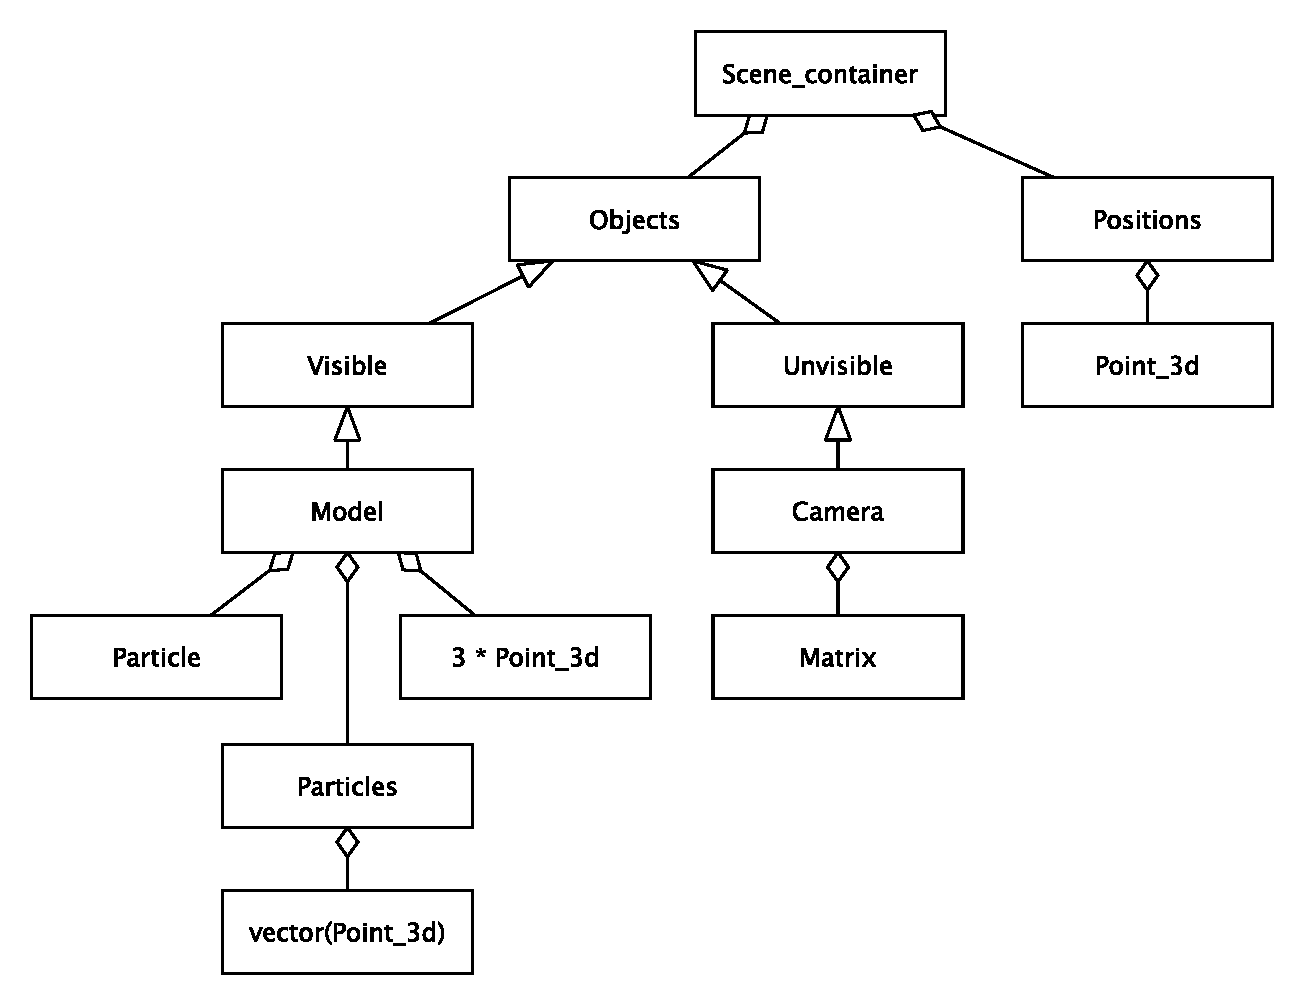
\includegraphics[scale=0.7]{scenecontainer.pdf}
	\caption{Контейнер сцены}
	\label{img:scenecontainer}
\end{figure}

Для создания сложной модели используется паттерн строитель. Для последовательного обхода объектов на сцене -- паттерн итератор. 

\section{\textbf{Требования к аппаратуре }}

Так как в данной работе используется трассировка лучей, в которой необходимо пробегаться по всем пикселям экрана, стоит необходимость уменьшения временных затрат на вычисления. 

Таким образом, существует необходимость использования параллельных вычислений. Так как параметры каждого пикселя экрана вычисляются независимо от других, то для того, чтобы вычислить все параллельно, достаточно просто указать какие пиксели какому потоку вычислять.

Теоретически, для нахождения значения каждого из пикслей можно создать свой поток. Но ОС не позволит создать такое число потоков, ресурсов на их создание не хватит и создание потока также занимает определенный промежуток времени.

Алгоритм. 
\begin{enumerate}
	\item Разделить экран по оси Х на равные участки N. 
	\item Создать N потоков с указанием вычисляемых пикселей. 
	\item Запустить потоки. 
\end{enumerate}

Проведено исследование с замером времени необходимого на отрисовку экрана для разного количества потоков. Количество повторов эксперимента -- 15.

\begin{table}[]
	\begin{tabular}{|c|l|l|l|l|l|}
	\hline
	\begin{tabular}[c]{@{}c@{}}Количество \\ потоков\end{tabular}                                  & 1           & 2       & 4          & 8          & 16         \\ \hline
	\begin{tabular}[c]{@{}c@{}}Среднее время \\ визуализации\\ экрана,\\ микросекунды\end{tabular} & 11518775.92 & 6013675 & 3298333.53 & 2843617.94 & 2886129.94 \\ \hline
	\end{tabular}
\end{table}

Как видно из эксперимента, наиболее быстрая отрисовка при количестве потоков равным 8, что равно количеству логических ядер процессора. 

Следовательно, для наиболее быстрой работе, количество логических ядер процессора на персональном компьютере должно быть больше 8. 

\section{\textbf{Требования к программному обеспечению }}

С помощью Qt можно создавать графические приложения на различных операционных системах, не переписывая исходный код. Qt поддерживается на различных 32-битных и 64-битных платформах. 

Qt -- кроссплатформенная библиотека разработки GUI на С++, а значит нет привязки к платформе, возможно использование любого ПО. 

Qt Creator доступен для следующих операционных систем:

\begin{enumerate}
	\item[1. ]Windows 7 или более поздняя версия
	\item[2. ]Ubuntu Linux 16.04 (64-разрядная версия) или более поздняя версия
	\item[3. ]macOS 10.12 или более поздней версии
\end{enumerate}

\section{\textbf{Порядок работы }}

Алгоритм программы. 

\begin{enumerate}
	\item[1. ] Визуализация начального экрана и интерфейса. 
	\item[2. ] Ввод и чтение из пользовательского файла. 
	\item[3. ] Если ошибок не возникло, загрузка новой модели. 
	\item[4. ] Визуализация модели с учетом матрицы камеры. 
	\begin{enumerate}
		\item Алгоритм трассировки для каждого пикселя экрана. 
		\item Определение затененности для каждого пикселя экрана. 
		\item Применение диффузного отражения для каждого пикселя экрана. 
		\item Отрисовка пикселей. 
	\end{enumerate}
	\item[5. ] При нажатой кнопке взрыва. 
	\begin{enumerate}
		\item Пересчет скорости каждого объекта по законам физики. 
		\item Пересчет положения каждого объекта с учетом скорости. 
	\end{enumerate}
	\item[6. ] Переход к пункту 4, если не загружен новый файл, иначе пункт 2. 
\end{enumerate}

\section{\textbf{Обращение к программе }}

Программа компилируется и запускается с помощью Qt Creator. 

Взаимодействие пользователя с приложением осуществляется через интерфейс, представленный на рисунке \ref{img:interface}. 

\section{\textbf{Входные и выходные данные }}

На вход поступают данные из файла, определенного вида. Также можно изменять данные с помощью графического интерфейса или менять направление камеры. 

На выходе получаем визуализацию столкновения частиц. 


\section{\textbf{Сообщения  системы }}

